\documentclass[journal]{IEEEtran}

% Packages
\usepackage{cite}
\usepackage{graphicx}
\usepackage{subfigure}
\usepackage{float}
\usepackage{url}
\usepackage{color}


\begin{document}

% paper title
% can use linebreaks \\ within to get better formatting as desired
\title{Autonomous~Robotics~Lab~2 \\ Building~a~Visibility~Graph~Using~RPS}
%

\author{Rodrigo~Caye~Daudt}





% make the title area
\maketitle



%%%%%%%%%%%%%%%%%%%%%%%%%%%%%%%%%%%%%%%%%%%%%%%%%%%%%%%%%%%%%%%%%%%%%%%%%%%%%%%
\section{Introduction}

\IEEEPARstart{T}{his} report describes the work done for lab 2 of the Autonomous Robotics module. The objective here was to develop a MATLAB function to apply the Rotational Plane Sweep (RPS) algorithm for building a visibility graph for a given topological map, which includes the starting point, the goal and the polygonal obstacles.

Section \ref{rps} describes in detail the RPS algorithm and gives some information about the developed implementation. Section \ref{results} contains the results and analysis for a few example environments. Section\ref{conclusion} concludes this work by highlighting the main points of this work.

%%%%%%%%%%%%%%%%%%%%%%%%%%%%%%%%%%%%%%%%%%%%%%%%%%%%%%%%%%%%%%%%%%%%%%%%%%%%%%%
\section{RPS Algorithm And Implementation}\label{rps}

As was previously mentioned, the Rotational Plane Sweep (RPS) algorithm's target is to build a visibility graph for a given topographical map. The input of the \textit{RPS} function is an $N \times 3$ matrix, where each row contains information about a vertex. The output of the function is an $M \times 2$ matrix, where each row contains the indices of a pair of vertices visible to each other. The first column contains the value of the X coordinate of each vertex, the second column contains the Y coordinate of each vertex, and the third column contains the index of the polygon to which the vertex belong. The starting point will always have polygon index 0, while the goal will have the highest polygon index and will be the only vertex to have that index. It is important that the vertices are given in order (either clockwise or counter-clockwise) and that no two edges have intersections other than the vertices they may share.

The idea behind RPS is to use an imaginary half-line with its origin at a given vertex and rotating it around that point to evaluate the visibility between that vertex and all other vertices in order of crossing this half-line. This method allows us to keep a list of active edges, which we will call the S list. This list enables the computer to check only a subset of the edges defined by the topographical map, speeding up the computations. At a given moment, the S list contain all the edges that may break the visibility line between two vertices, and all edges that are not present in the S list will not be considered at this step. The half-line starts at $0^{\circ}$ and it completes a full rotation around the origin vertex to evaluate all possible connections.

On this implementation, two additional structures were created at the beginning of the algorithm to facilitate the computations. The first structure is the list of all edges defined by the topographical map. This is extracted from the list of vertices, taking into account their order and to which polygon they belong. The edges are stored in the form \textit{[x1 y1 x2 y2]}, where each value defines the X or Y coordinates for each of the two vertices that define that edge. The second structure, which is created in parallel with the first one, is the indices of the edges in the edge list that are connected to each vertex. These structures allow us to calculate these values only once, while they would have to be calculated many times and in more complex ways if these structures were not stored at dedicated matrices.

The RPS algorithm is the application of the methods described in the following paragraphs to each vertex in the topographical map. By applying these steps to all vertices we are able to find all visibility lines and to construct a visibility graph based on the RPS results.

The first step in the RPS algorithm is to calculate the angles from the current considered vertex, which we will call $v$, to every other vertex in the map, which we will call $v_i$. The sorting of this list will allow the RPS to start at the $0^{\circ}$ half-line and to stop at the crossings with each $v_i$ in rotational order.

The next step is to initialize the S list with all the edges which are intersected by the horizontal half-line since those are the relevant edges at that angle. This is done by looping through all the edges contained in the edge list structure that was previously created. All edges must be checked at this point. The intersections between lines were calculated using the MATLAB function \textit{polyxpoly}, which returns the coordinates of any crossings between the lines of two "polylines".

The next step in the algorithm is to loop through all the other vertices $v_i$ and to check their visibility. As was mentioned before, only the edges contained in the S list at that moment are considered for the visibility calculations. This reduced number of considered edges is the reason RPS is a good algorithm for building visibility graphs, since it runs much faster than brute force methods, especially for larger topographical maps.

For each other vertex $v_i$ it is also important to update the S list. If $v_i$ is the beginning of an edge not currently in S that edge should be added, and if it is the end of an edge currently in S that edge should be removed from S.

Two main concerns arise from this implementation of RPS and should be dealt with. The first one is that edges will be found twice. For example if \textit{[i j]} is a valid edge, then \textit{[j i]} is also a valid edge, but it is meaningless to have both present in the final visibility graph. Therefore, before adding visible connections to the visibility graph we should check if its mirrored version is already in the list.

The second concern is that since visibility is determined solely based on intersections with edges, connections inside polygons are initially allowed. These connections should be removed from the final visibility graph, since they are not valid paths that can be used for path planning. To find out if a visivility line is inside a given polygon, the MATLAB function \textit{inpolygon} was used to evaluate the central point of the visibility line. The line was kept in the visibility graph if the central point was outside the polygon or on one of its edges, and it was removed if the point was inside its boundaries. It should be noted that connexions along polygon edges should be kept, since they are still valid path segments.




%\begin{figure}
%	\centering
%	\includegraphics[width=0.8\linewidth]{figures/blocks.png}
%	\caption{Illustration }
%	\label{blocks}
%\end{figure}








%%%%%%%%%%%%%%%%%%%%%%%%%%%%%%%%%%%%%%%%%%%%%%%%%%%%%%%%%%%%%%%%%%%%%%%%%%%%%%%
\section{Tests and Results}\label{results}

The developed \textit{RPS} function was tested using several different environments. Some of these environments and the results are shown in Fig. \ref{fig:results}, where four different environments were used to exemplify different possible situations.

\begin{figure*}[p]
	\centering
	\subfigure[Environment 1]{\label{e1c}
		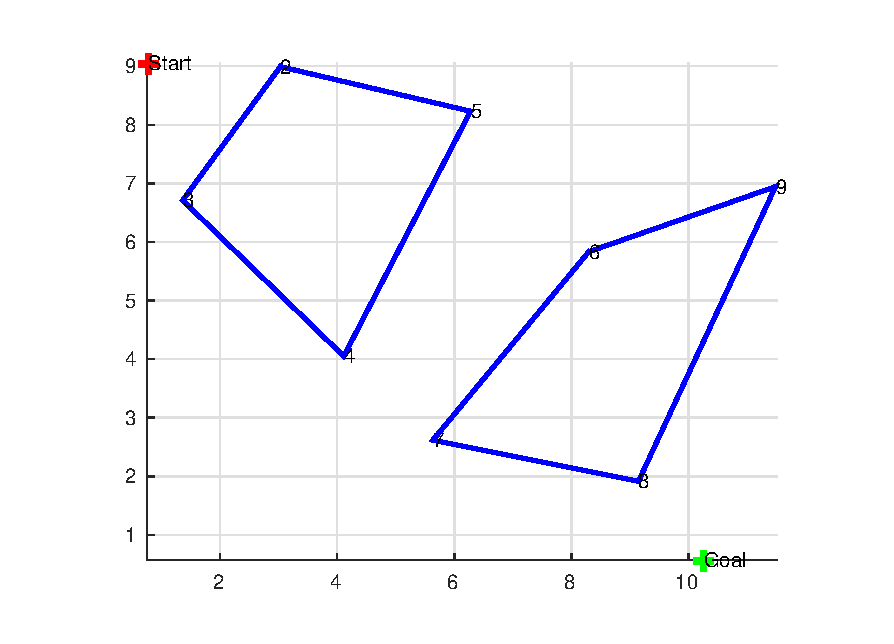
\includegraphics[width=0.35\linewidth]{figures/e1c.eps}}~
	\subfigure[Visibility graph for environment 1]{\label{e1s}
		\includegraphics[width=0.35\linewidth]{figures/e1s.eps}}\\
	
	\subfigure[Environment 2]{\label{e2c}
		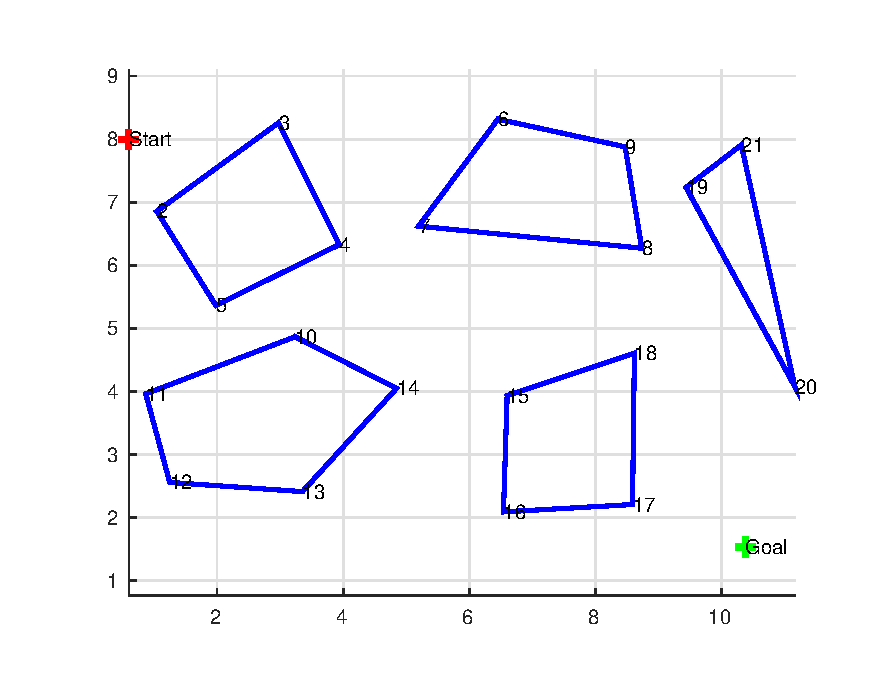
\includegraphics[width=0.35\linewidth]{figures/e2c.eps}}~
	\subfigure[Visibility graph for environment 2]{\label{e2s}
		\includegraphics[width=0.35\linewidth]{figures/e2s.eps}}\\
	
	\subfigure[Environment 3]{\label{e3c}
		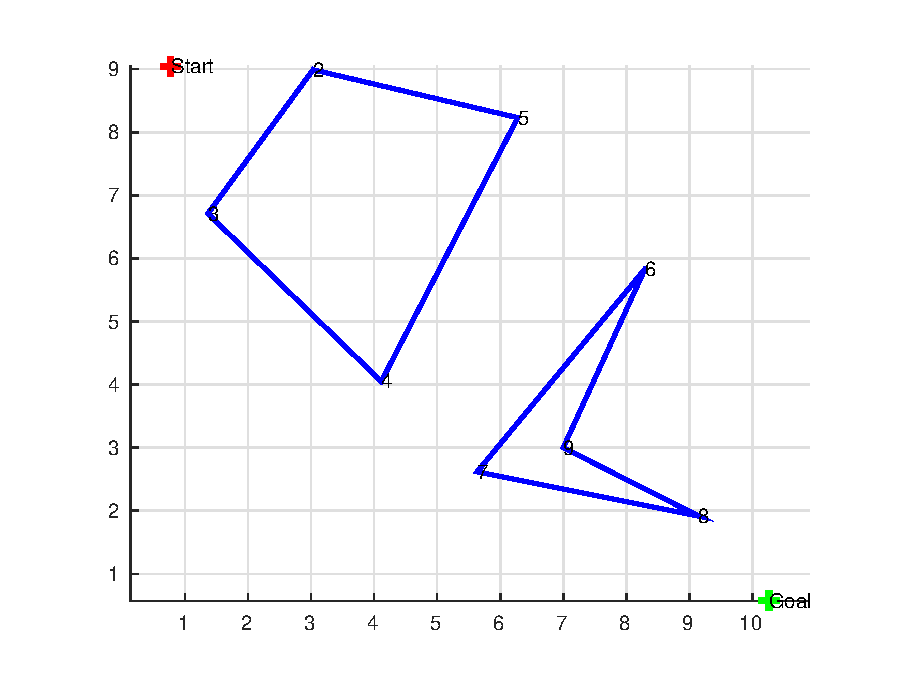
\includegraphics[width=0.35\linewidth]{figures/e3c.eps}}~
	\subfigure[Visibility graph for environment 3]{\label{e3s}
		\includegraphics[width=0.35\linewidth]{figures/e3s.eps}}\\

	\subfigure[Environment 4]{\label{e4c}
		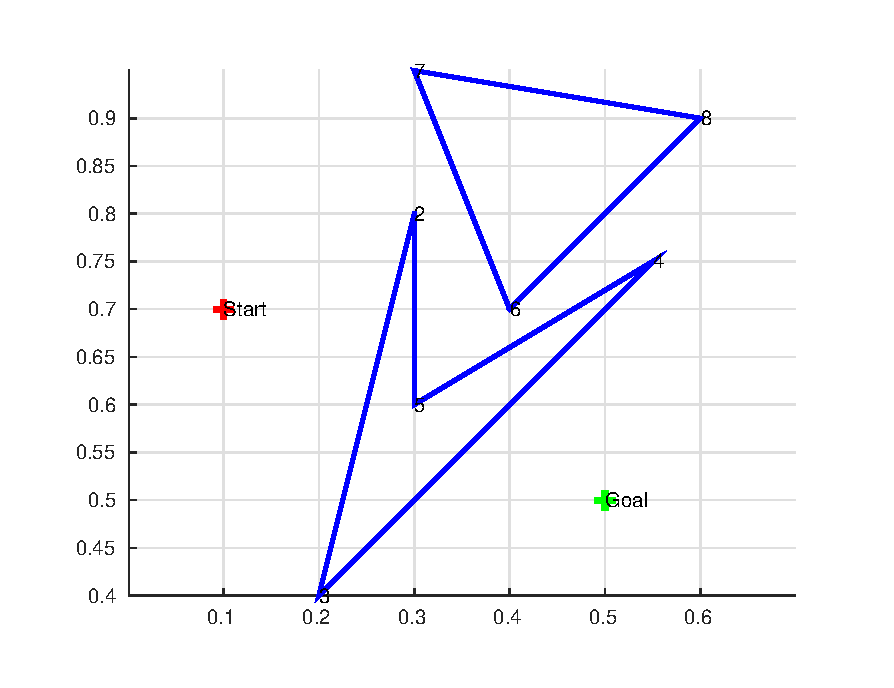
\includegraphics[width=0.35\linewidth]{figures/e4c.eps}}~
	\subfigure[Visibility graph for environment 4]{\label{e4s}
		\includegraphics[width=0.35\linewidth]{figures/e4s.eps}}
		
	\caption{RPS results for different environments}
	\label{fig:results}
\end{figure*}

Figure \ref{e1c} shows a simple environment containing only two convex polygons as obstacles. In this image, as in all the others, the obstacles are defined by the blue lines, the start point is displayed as a red cross and the goal is displayed as a green cross. The number of each vertex and text labels for Start and Goal are also displayed in the appropriate locations. In Fig. \ref{e1s} we see the result from the \textit{RPS} function, where the lines in red represent the visible connexions between vertices of the topographical map. We can see that, as expected, only visible vertices are connected to each other, the edges of the polygons are considered valid connexions, and no visibility is considered inside the polygons.

Figures \ref{e2c} and \ref{e2s} show the raw environment and the result using a more complex set of polygons. This example shows that the RPS algorithm can be applied for any number of obstacles without problem.

Figure \ref{e3c} shows a variation of the environment shown in Fig. \ref{e1c}, where polygon two has been turned into a non-convex polygon. We can see in Fig. \ref{e3s} that the developed \textit{RPS} function works well with non-convex polygons, as now vertex 6 is connected to vertex 8. The function is able to tell if a given connexion is inside the polygon 

Figure \ref{e4c} shows the final example environment, which contains a non-convex polygon but a different polygon is partially inside its concavity. The result is displayed in Fig. \ref{e4s}, and we can see that once again the \textit{RPS} function correctly calculated the visibility graph even for a complex case like this. Vertices 2 and 4 were not connected since polygon 2 obstructed their connexion.

One limitation of the developed \textit{RPS} function is that it is unable to deal with holes in the considered obstacles. This limitation comes from the way the inputs are formatted, which doesn't allow for the description of shapes with holes. This could be solved by coupling the developed \textit{RPS} function with an input sanitizing function which would remove the holes from the obstacles. This loss of information would not affect the calculated trajectory since the trajectories can only go outside the objects. This sanitizing function could also be used to make sure that the input is adequate, i.e. the starting point is the only vertex in polygon 0, the goal is the only vertex in its polygon index, and there are no crossing edges defined by the vertex list.

%%%%%%%%%%%%%%%%%%%%%%%%%%%%%%%%%%%%%%%%%%%%%%%%%%%%%%%%%%%%%%%%%%%%%%%%%%%%%%%
\section{Conclusion}\label{conclusion}

This report described in general terms on Section \ref{rps} the RPS algorithm and gave some information about its implementation for this work, as well as the motivation to use the RPS algorithm for path planning. In Section \ref{results} some results of the developed \textit{RPS} function were displayed and analysed, and we concluded that the written function works for all possible cases as long as the inputs are appropriate.

The RPS algorithm proved to be a fast path planning algorithm for situations where topographical maps of the environment are available. The results in Fig. \ref{fig:results} indicate that it is a very robust algorithm and can be applied in a wide variety of maps.



%\bibliographystyle{IEEEtran}
%\bibliography{Template_Daudt}


\end{document}


